\documentclass{article}
\usepackage{graphicx}
\usepackage{caption}
\usepackage{subcaption}
\usepackage{hyperref}
\graphicspath{{./figs/}}{}
\usepackage{listings}
\title{
HLS-Assignment 9 PART-1
}
\begin{document}
\maketitle
\hfill \textbf{Sampath Govardhan} \\
\null \hfill \textbf{FWC22071}\\
\maketitle
\hfill \textbf{VITIS-HLS}
\section{Problem Statement}
\href{run:./problem_statement.pdf} {Problem Statemt}
\vspace{1cm}
\section{Header File}
\begin{lstlisting}
//header.h
#ifndef _HEADER_H_
#define _HEADER_H_

#include <hls_stream.h>
#include "ap_int.h"
using namespace std;

#define N 8      //length of input message
#define y 25     //length of divisor(parity)
#define x N+y-1  //length of crc (len of input+divisor-1)

typedef ap_uint<N> data;


void crc24a(hls::stream<data>& input, hls::stream<data>& output);

#endif



\end{lstlisting}

\vspace{15cm}
\section{CRC bits Generator Code}
\begin{lstlisting}
//crc.cpp
#include "header.h"

void crc24a(hls::stream<data>& input, hls::stream<data>& output) {

#pragma HLS INTERFACE mode=axis register_mode=both port=input register
#pragma HLS INTERFACE mode=axis register_mode=both port=output register

	ap_uint<1> crc[x],oput[x];
    ap_uint<1> divisor[y] = {1, 1, 0, 0, 0, 0, 1, 1, 0, 0, 1, 0, 0, 1, 1, 0, 0, 1,
    1, 1, 1, 1, 0, 1, 1};
    data o1,o2,o3,o4;

// Read input stream and do padding
    data d = input.read();
   loop1: for (int i = 0; i < x; i++) {
#pragma HLS UNROLL
    	crc[i] = (i < N) ? d(i,i) : 0;
    	oput[i] = (i < N) ? d(i,i) : 0;
    }
   ap_uint<1> last=input.read();

// Division is performed only when last is high
   loop2: for (int i = 0; i <= x - y; i++) {
#pragma HLS PIPELINE II=1
        if (crc[i] == 1 && last==1) {
          loop3:  for (int j = 0; j < y; j++) {
        	  int k=i+j;
#pragma HLS UNROLL
                crc[k] = crc[k] ^ divisor[j];
            }
        }
    }

// Write the result to output stream c

   loop4:for (int i = 0; i < x; i++) {
#pragma HLS UNROLL
	   oput[i] = crc[i] ^ oput[i];
       if (i < N) {
           o1(i, i) = oput[i];
       }else if (i < N * 2){
           o2(i % N, i % N) = oput[i];
       } else if (i < N * 3) {
           o3(i % N, i % N) = oput[i];
       } else {
           o4(i % N, i % N) = oput[i];
       }
   }

   output.write(o1);
   output.write(o2);
   output.write(o3);
   output.write(o4);
}

\end{lstlisting}
\vspace{2cm}

\section{Test Bench Code}
\begin{lstlisting}
//crc_tb.cpp
#include "header.h"
#include <vector>
int main() {
    hls::stream<data> a,b;
    data w;
    ap_uint<1> last;

      w=0b00010110;                                               //msbtolsb

          /* ap_uint<1> dividend[8] = {0, 1, 1, 0, 1, 0, 0, 0};   //lsbtomsb
   	       for (int i = 0; i < 8; i++) {

   	              w(i,i) = dividend[i];

   	              }
   	      */
          last=1;
   	       a.write(w);
   	       a.write(last);




// Perform binary divison
    crc24a(a, b);

// Read the result from the output stream
    vector<ap_uint<1>> p;
    cout << "CRC generator output : ";
    while(!b.empty()){
          data d = b.read();
         for (int i = 0; i < N ; i++) {
          	cout<< d(i,i);
          	p.push_back(d(i,i));
          }
       }
       cout<<endl;

// Checking if output is valid or not
           bool flag=0;
           ap_uint<1> divisor[y] = {1, 1, 0, 0, 0, 0, 1, 1, 0, 0, 1, 0, 0, 1, 1, 0,
           0, 1, 1, 1, 1, 1, 0, 1, 1};


       //Output is valid only when remainder divison of output with divisor is 0
           for (int i = 0; i <= x - y; i++) {
               if (p[i] == 1) {
                   for (int j = 0; j < y; j++) {
                       p[i + j] = p[i+j] ^ divisor[j];
                   }
               }
           }
           cout<<"CRC detector output :  ";
           for (int i = 0; i < 32; i++) {
           	cout<<p[i];
               if (p[i]==1){
               	flag=1;
               }
           }
            cout<<endl;
           if ( flag==0) {
                      cout << "!PASS!CRC Check at detector is Success" << endl;
                  }
           else {
                      cout << "!ERROR!CRC Check at detector has Failed" << endl;
                  }
    return 0;
}

\end{lstlisting}
\vspace{13cm}


\section{C simulation Output}
\begin{lstlisting}
INFO: [SIM 2] *************** CSIM start ***************
INFO: [SIM 4] CSIM will launch GCC as the compiler.
   Compiling ../../../../codes/crc_tb.cpp in debug mode
   Generating csim.exe
CRC generator output : 01101000101101001111001100000010
CRC detector output :  00000000000000000000000000000000
!PASS!CRC Check at detector is Success
INFO [HLS SIM]: The maximum depth reached by any hls::stream() instance in the
design is 4
INFO: [SIM 1] CSim done with 0 errors.
INFO: [SIM 3] *************** CSIM finish ***************




\end{lstlisting}
\vspace{15cm}

\section{HLS Resource Consumption Report}
\vspace{1cm}
\begin{figure}[h]
\centering
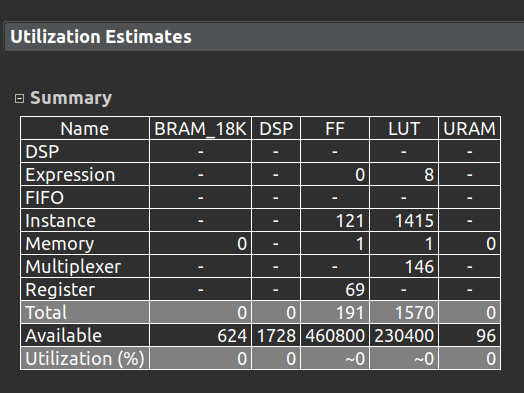
\includegraphics[width=\textwidth]{figs/p11.png}
    \caption{Resource Consumption}
    \label{fig:my_label}
\end{figure}

\vspace{13cm}


\section{HLS Timing and Fmax Report}
\vspace{1cm}
\begin{figure}[h]
    \centering
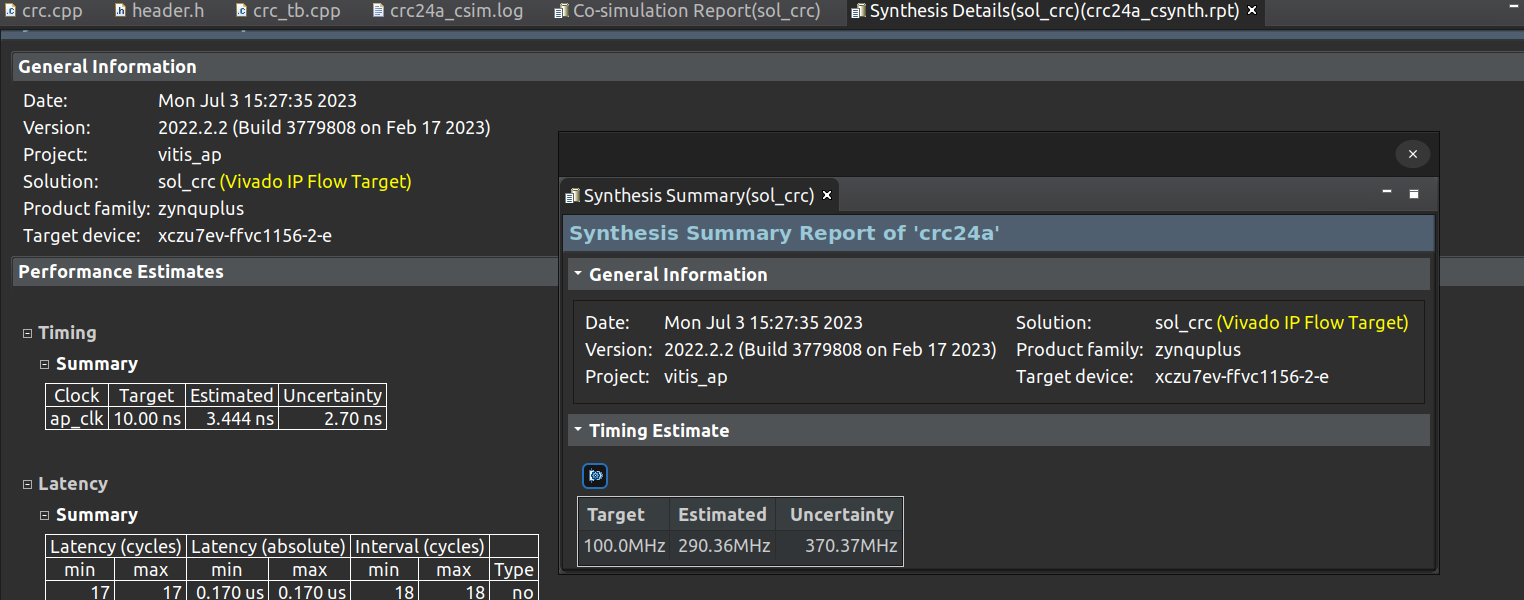
\includegraphics[width=1.4\textwidth]{figs/p12.png}
    \caption{Timing and Fmax}
    \label{fig:my_label}
\end{figure}

\vspace{15cm}


\section{CoSimulation Report}
\vspace{1cm}
\begin{figure}[h]
    \centering
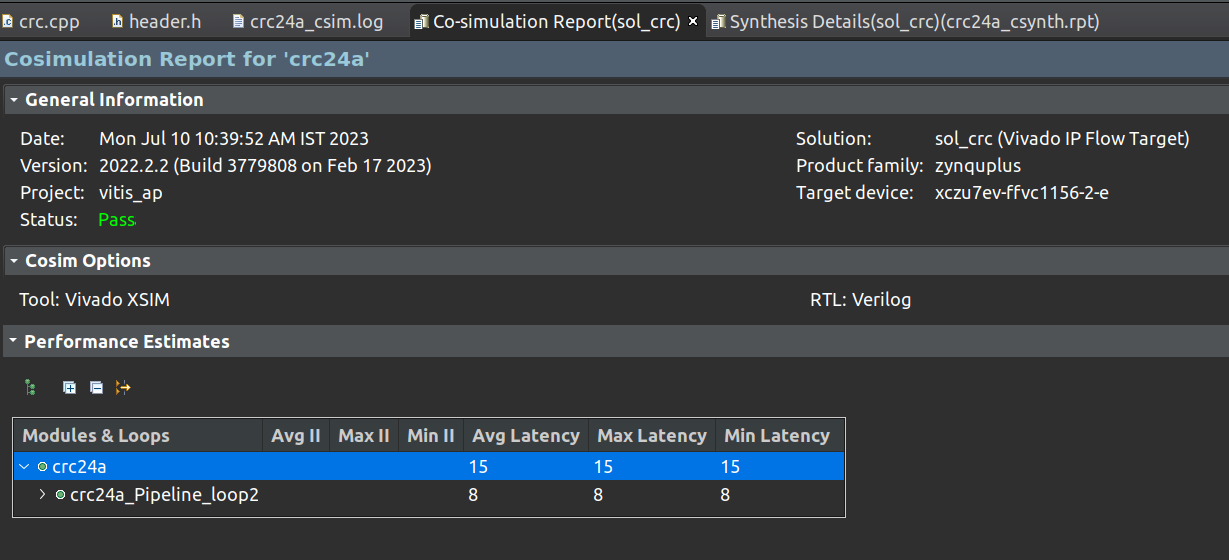
\includegraphics[width=1.4\textwidth]{figs/p13.png}
    \caption{Cosimulation}
    \label{fig:my_label}
\end{figure}

\vspace{15cm}


\maketitle
\hfill \textbf{VIVADO}
\section{Block Design}
\vspace{1cm}
\begin{figure}[h]
    \centering
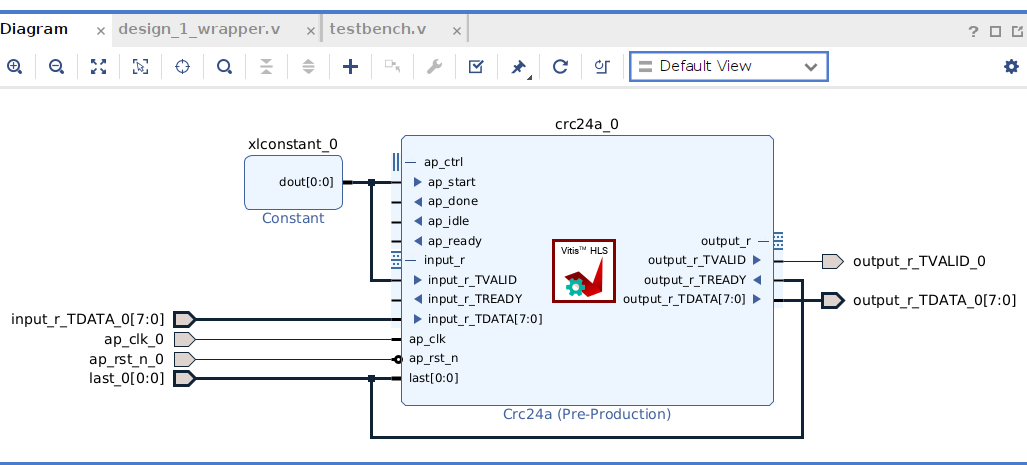
\includegraphics[width=\columnwidth]{figs/p1bd.png}
    \caption{Block Diagram}
    \label{fig:my_label}
\end{figure}
\vspace{3cm}
\section{Verilog Testbench}
\begin{lstlisting}
//testbench.v
`timescale 1ns / 1ps
//////////////////////////////////////////////////////////////////////////////////
// Company: 
// Engineer: 
// 
// Create Date: 06/26/2023 11:35:30 AM
// Design Name: 
// Module Name: testbench
// Project Name: 
// Target Devices: 
// Tool Versions: 
// Description: 
// 
// Dependencies: 
// 
// Revision:
// Revision 0.01 - File Created
// Additional Comments:
// 
//////////////////////////////////////////////////////////////////////////////////


module testbench();
        reg ap_clk_0;
        reg ap_rst_n_0;
        always #5 ap_clk_0=~ap_clk_0;
        
        reg [7:0] ip;
        wire [7:0] op;
        wire output_r_TVALID_0;
       
        initial begin
        ap_clk_0=0;ap_rst_n_0=0;
        #10
        ap_rst_n_0=1;
        #10
        ip=8'b00010110;//ascii "h"
        #10
        ip=8'b00000001;
        #200
        $finish;
        end
      design_1_wrapper uut(.ap_clk_0(ap_clk_0), .ap_rst_n_0(ap_rst_n_0),
      .input_r_TDATA_0(ip),.output_r_TDATA_0(op),
      .output_r_TVALID_0(output_r_TVALID_0));
    
    
endmodule

\end{lstlisting}

\vspace{3cm}


\section{Output Waveform}
\vspace{1cm}
\begin{figure}[h]
\centering
\begin{subfigure}[b]{1.1\textwidth}
    \centering
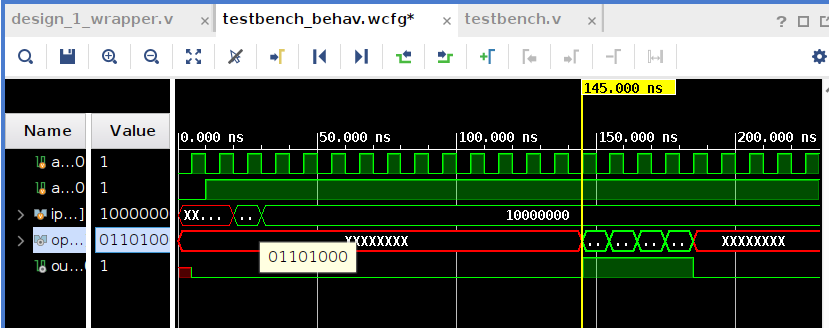
\includegraphics[width=\textwidth]{figs/p1wavfull.png}
    \caption{Output of IP}
    \label{fig:my_label}
\end{subfigure}
\hfill
\begin{subfigure}[b]{1.1\textwidth}
    \centering
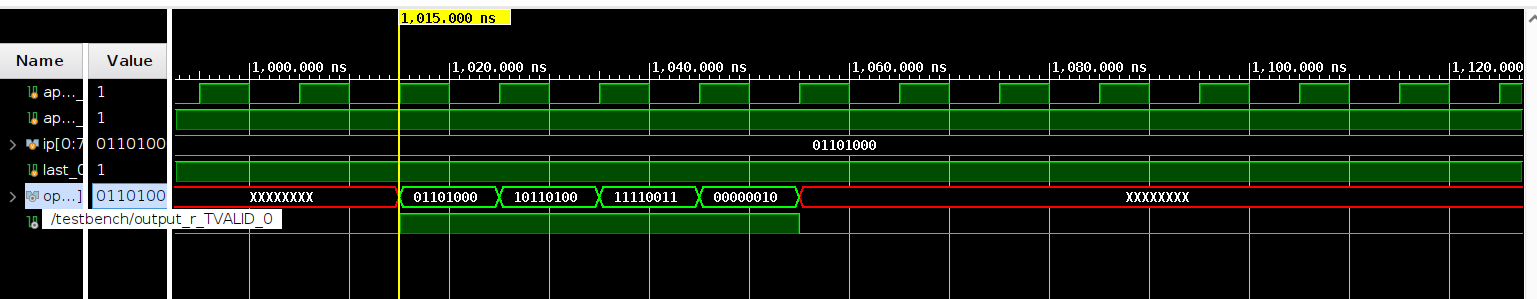
\includegraphics[width=\textwidth]{figs/p1wav.png}
    \caption{Zoomed format of above figure}
    \label{fig:my_label}
\end{subfigure}
\end{figure}
\vspace{13cm}

\section{Design Choices}
\begin{lstlisting}

1. Initially I had designed the code with input message stream of unknown length 
up to a maximum of 1024,whenever input stream reads a value of 1, until then all
values are stored in a array and then binary division takes place.(code is 
uploaded in github named dummy.cpp is in codes folder along with all other codes)

2. This code compiles successfully, but while synthesis it gives an error
"unsupported memory access on variable 'vla211' which is (or contains) an array
with unknown size at compile time".

3. Since hls does not support dynamic memory allocation and arrays should be of
fixed length so Initally I took input message length as a fixed variable with 8
bits and continued with the problem accordingly.

4. By using above aspects in point3 I designed the cyclic redundancy check
generator module in HLS.

\end{lstlisting}
\vspace{1cm}

\end{document}


